\chapter{Naughty maid}
Naughty maid is the adult theme app name of the remaining four malware samples analyzed. The objective of the virus is to log to a remote chinese server sensitive information like position and stored files and, in addition, can make the phone subscribe to paid SMS services  and cancel the SMS afterwards to hide its malicious behavior.

\section{File differences}
As previously stated we received four jar files identified by their SHA256 hash:
\begin{itemize}
	\item \texttt{0b8bae30da84fb181a9ac2b1dbf77eddc5728fab8dc5db44c11069fef1821ae6}
	\item \texttt{0b41181a6b9c85b8fa5c8e8c836ac24dd6e738a0d843f0b81b46ffe41b925818}
	\item \texttt{0c05e5035951e260725d15392c8792a4941f92f868558e8b90b52977d832a70d}
	\item \texttt{0c40fb505fb96ca9aed220f48a3c6c22318d889efa62bc7aaeee98f3a740afab}
\end{itemize}
 
To make sure they were part of the same family of viruses, we used a jar compare tool confirming that most of the source files were practically identical. Only \texttt{0c05..} presented slightly more differences, mainly in the \texttt{AndroidManifest.xml} file, but otherwise remained the same w.r.t. the other files (Fig. \ref{fig:jarCompare}).

\begin{figure}[h!]
\centering
    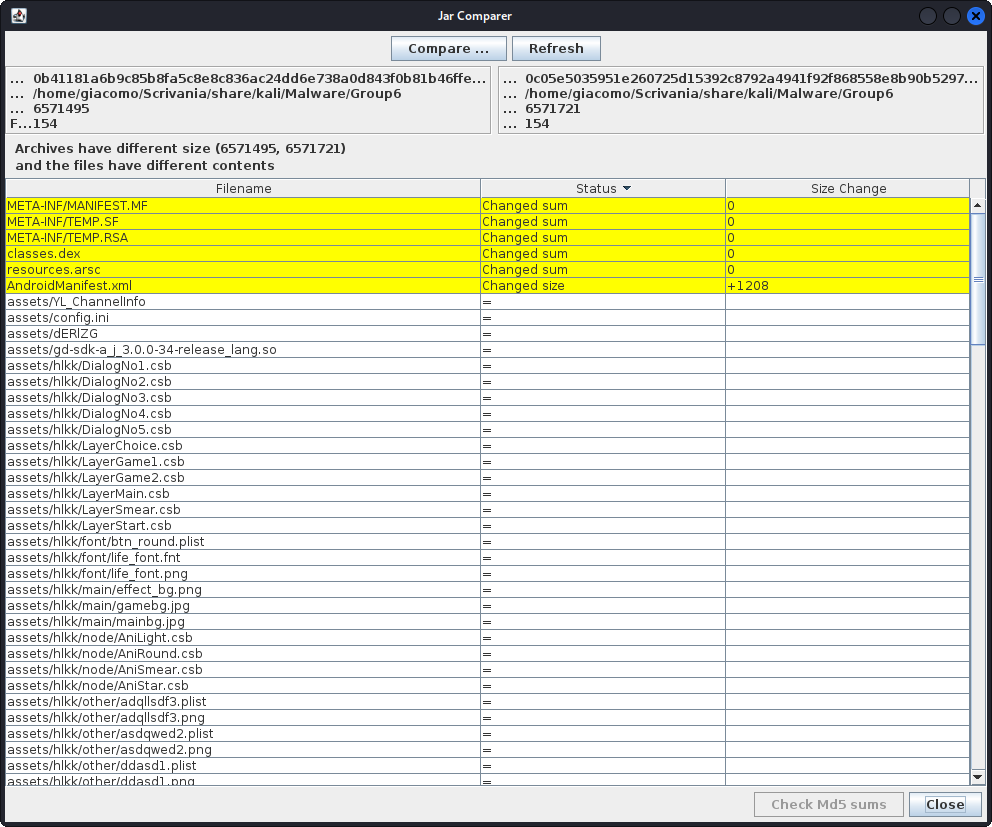
\includegraphics[width=1\textwidth]{./images/screenshot/jarcompare/jarCompare.png}
    \caption{jarCompare output}
    \label{fig:jarCompare}
\end{figure}

From this point forward we will always reference the \texttt{0c05..} sample file and its content when speaking about this virus family and, if there will be any differences with the other samples, they will be pointed out.

\section{Static Analysis}

As with SanaSystem, we firstly fed the obtained APK to virus total and got the following result shown in Fig. \ref{fig:MaidReview}.
\begin{figure}[h!]
\centering
    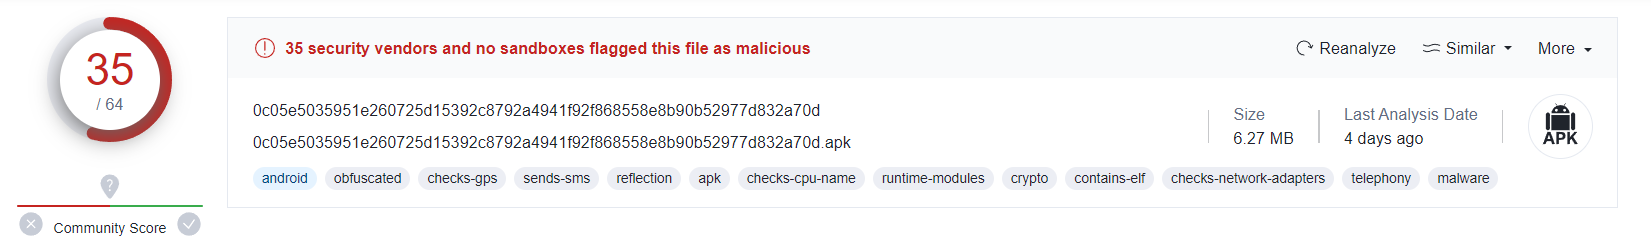
\includegraphics[width=1\textwidth]{./images/screenshot/NaughtyMaid/Review.png}
    \caption{Virus total review}
    \label{fig:MaidReview}
\end{figure}

In addition, the \texttt{0c40..} file received a score of 33/59, this indicates that, even if the files are practically the same, even small changes can affect the malware fingerprint which changes its detectability from anti-viruses. In particular a common anti-malware such as MalwareBytes was not able to recognize the software as malicious in every case.